\documentclass[twoside]{book}

% Packages required by doxygen
\usepackage{fixltx2e}
\usepackage{calc}
\usepackage{doxygen}
\usepackage[export]{adjustbox} % also loads graphicx
\usepackage{graphicx}
\usepackage[utf8]{inputenc}
\usepackage{makeidx}
\usepackage{multicol}
\usepackage{multirow}
\PassOptionsToPackage{warn}{textcomp}
\usepackage{textcomp}
\usepackage[nointegrals]{wasysym}
\usepackage[table]{xcolor}

% Font selection
\usepackage[T1]{fontenc}
\usepackage[scaled=.90]{helvet}
\usepackage{courier}
\usepackage{amssymb}
\usepackage{sectsty}
\renewcommand{\familydefault}{\sfdefault}
\allsectionsfont{%
  \fontseries{bc}\selectfont%
  \color{darkgray}%
}
\renewcommand{\DoxyLabelFont}{%
  \fontseries{bc}\selectfont%
  \color{darkgray}%
}
\newcommand{\+}{\discretionary{\mbox{\scriptsize$\hookleftarrow$}}{}{}}

% Page & text layout
\usepackage{geometry}
\geometry{%
  a4paper,%
  top=2.5cm,%
  bottom=2.5cm,%
  left=2.5cm,%
  right=2.5cm%
}
\tolerance=750
\hfuzz=15pt
\hbadness=750
\setlength{\emergencystretch}{15pt}
\setlength{\parindent}{0cm}
\setlength{\parskip}{3ex plus 2ex minus 2ex}
\makeatletter
\renewcommand{\paragraph}{%
  \@startsection{paragraph}{4}{0ex}{-1.0ex}{1.0ex}{%
    \normalfont\normalsize\bfseries\SS@parafont%
  }%
}
\renewcommand{\subparagraph}{%
  \@startsection{subparagraph}{5}{0ex}{-1.0ex}{1.0ex}{%
    \normalfont\normalsize\bfseries\SS@subparafont%
  }%
}
\makeatother

% Headers & footers
\usepackage{fancyhdr}
\pagestyle{fancyplain}
\fancyhead[LE]{\fancyplain{}{\bfseries\thepage}}
\fancyhead[CE]{\fancyplain{}{}}
\fancyhead[RE]{\fancyplain{}{\bfseries\leftmark}}
\fancyhead[LO]{\fancyplain{}{\bfseries\rightmark}}
\fancyhead[CO]{\fancyplain{}{}}
\fancyhead[RO]{\fancyplain{}{\bfseries\thepage}}
\fancyfoot[LE]{\fancyplain{}{}}
\fancyfoot[CE]{\fancyplain{}{}}
\fancyfoot[RE]{\fancyplain{}{\bfseries\scriptsize Generated by Doxygen }}
\fancyfoot[LO]{\fancyplain{}{\bfseries\scriptsize Generated by Doxygen }}
\fancyfoot[CO]{\fancyplain{}{}}
\fancyfoot[RO]{\fancyplain{}{}}
\renewcommand{\footrulewidth}{0.4pt}
\renewcommand{\chaptermark}[1]{%
  \markboth{#1}{}%
}
\renewcommand{\sectionmark}[1]{%
  \markright{\thesection\ #1}%
}

% Indices & bibliography
\usepackage{natbib}
\usepackage[titles]{tocloft}
\setcounter{tocdepth}{3}
\setcounter{secnumdepth}{5}
\makeindex

% Hyperlinks (required, but should be loaded last)
\usepackage{ifpdf}
\ifpdf
  \usepackage[pdftex,pagebackref=true]{hyperref}
\else
  \usepackage[ps2pdf,pagebackref=true]{hyperref}
\fi
\hypersetup{%
  colorlinks=true,%
  linkcolor=blue,%
  citecolor=blue,%
  unicode%
}

% Custom commands
\newcommand{\clearemptydoublepage}{%
  \newpage{\pagestyle{empty}\cleardoublepage}%
}

\usepackage{caption}
\captionsetup{labelsep=space,justification=centering,font={bf},singlelinecheck=off,skip=4pt,position=top}

%===== C O N T E N T S =====

\begin{document}

% Titlepage & ToC
\hypersetup{pageanchor=false,
             bookmarksnumbered=true,
             pdfencoding=unicode
            }
\pagenumbering{alph}
\begin{titlepage}
\vspace*{7cm}
\begin{center}%
{\Large Va\+Exception \\[1ex]\large 17.\+01.\+09 }\\
\vspace*{1cm}
{\large Generated by Doxygen 1.8.13}\\
\end{center}
\end{titlepage}
\clearemptydoublepage
\pagenumbering{roman}
\tableofcontents
\clearemptydoublepage
\pagenumbering{arabic}
\hypersetup{pageanchor=true}

%--- Begin generated contents ---
\chapter{Va\+Exception Documentation}
\label{index}\hypertarget{index}{}A little more convinient tool for throwing exceptions. \begin{DoxyParagraph}{Version}
17.\+01.\+09 
\end{DoxyParagraph}
\begin{DoxyParagraph}{Copyright}
(C) Vladislav Aleinik (\href{mailto:valeinik00@gmail.com}{\tt valeinik00@gmail.\+com}) 
\end{DoxyParagraph}
\begin{DoxyParagraph}{Date}
2017-\/01-\/09 22\+:13\+:37 +0400
\end{DoxyParagraph}


\begin{DoxyParagraph}{What is Va\+Exception?}
Va\+Exception (Vladik Aleinik Exception) is just like std\+::exception, but it gives more information on the error (it allows you to pass line, function and file, in which the exception was thrown). To learn more watch \hyperlink{class_va_exc_1_1_exception}{Va\+Exc\+::\+Exception} docs.
\end{DoxyParagraph}
\begin{DoxyWarning}{Warning}
Va\+Exception is currently (and forever) in alpha state, so bugs can occur. 
\end{DoxyWarning}

\chapter{Namespace Index}
\section{Namespace List}
Here is a list of all documented namespaces with brief descriptions\+:\begin{DoxyCompactList}
\item\contentsline{section}{\hyperlink{namespace_va_exc}{Va\+Exc} \\*Namespace with the whole code }{\pageref{namespace_va_exc}}{}
\item\contentsline{section}{\hyperlink{namespace_va_exc_1_1__control}{Va\+Exc\+::\+\_\+control} \\*Control over program behavior }{\pageref{namespace_va_exc_1_1__control}}{}
\item\contentsline{section}{\hyperlink{namespace_va_exc_1_1__error_info}{Va\+Exc\+::\+\_\+error\+Info} \\*Namespace for \hyperlink{class_va_exc_1_1__error_info_1_1_error_info}{Error\+Info} struct to store information conviniently (not for user) }{\pageref{namespace_va_exc_1_1__error_info}}{}
\item\contentsline{section}{\hyperlink{namespace_va_exc_1_1__literals}{Va\+Exc\+::\+\_\+literals} \\*User-\/defined literals for convinient wrapping }{\pageref{namespace_va_exc_1_1__literals}}{}
\item\contentsline{section}{\hyperlink{namespace_va_exc_1_1__wrappers}{Va\+Exc\+::\+\_\+wrappers} \\*Wrappers to be used in \hyperlink{class_va_exc_1_1_exception}{Exception} constructor (Exception()), mostly not for user use }{\pageref{namespace_va_exc_1_1__wrappers}}{}
\end{DoxyCompactList}

\chapter{Hierarchical Index}
\section{Class Hierarchy}
This inheritance list is sorted roughly, but not completely, alphabetically\+:\begin{DoxyCompactList}
\item \contentsline{section}{Va\+Exc\+:\+:\+\_\+wrappers\+:\+:Arg\+Filename}{\pageref{struct_va_exc_1_1__wrappers_1_1_arg_filename}}{}
\item \contentsline{section}{Va\+Exc\+:\+:\+\_\+wrappers\+:\+:Arg\+Function}{\pageref{struct_va_exc_1_1__wrappers_1_1_arg_function}}{}
\item \contentsline{section}{Va\+Exc\+:\+:\+\_\+wrappers\+:\+:Arg\+Line}{\pageref{struct_va_exc_1_1__wrappers_1_1_arg_line}}{}
\item \contentsline{section}{Va\+Exc\+:\+:\+\_\+wrappers\+:\+:Arg\+Msg}{\pageref{struct_va_exc_1_1__wrappers_1_1_arg_msg}}{}
\item \contentsline{section}{Va\+Exc\+:\+:\+\_\+wrappers\+:\+:Arg\+Msg\+Constexpr}{\pageref{struct_va_exc_1_1__wrappers_1_1_arg_msg_constexpr}}{}
\item \contentsline{section}{Va\+Exc\+:\+:\+\_\+error\+Info\+:\+:Error\+Info}{\pageref{class_va_exc_1_1__error_info_1_1_error_info}}{}
\item exception\begin{DoxyCompactList}
\item \contentsline{section}{Va\+Exc\+:\+:Exception}{\pageref{class_va_exc_1_1_exception}}{}
\end{DoxyCompactList}
\end{DoxyCompactList}

\chapter{Class Index}
\section{Class List}
Here are the classes, structs, unions and interfaces with brief descriptions\+:\begin{DoxyCompactList}
\item\contentsline{section}{\hyperlink{struct_va_exc_1_1__wrappers_1_1_arg_filename}{Va\+Exc\+::\+\_\+wrappers\+::\+Arg\+Filename} \\*Wrapper to store filename of the file in which \hyperlink{class_va_exc_1_1_exception}{Exception} is created }{\pageref{struct_va_exc_1_1__wrappers_1_1_arg_filename}}{}
\item\contentsline{section}{\hyperlink{struct_va_exc_1_1__wrappers_1_1_arg_function}{Va\+Exc\+::\+\_\+wrappers\+::\+Arg\+Function} \\*Wrapper to store function name in which \hyperlink{class_va_exc_1_1_exception}{Exception} is created }{\pageref{struct_va_exc_1_1__wrappers_1_1_arg_function}}{}
\item\contentsline{section}{\hyperlink{struct_va_exc_1_1__wrappers_1_1_arg_line}{Va\+Exc\+::\+\_\+wrappers\+::\+Arg\+Line} \\*Wrapper to store call line number in which \hyperlink{class_va_exc_1_1_exception}{Exception} is created }{\pageref{struct_va_exc_1_1__wrappers_1_1_arg_line}}{}
\item\contentsline{section}{\hyperlink{struct_va_exc_1_1__wrappers_1_1_arg_msg}{Va\+Exc\+::\+\_\+wrappers\+::\+Arg\+Msg} \\*Wrapper that stores exception message }{\pageref{struct_va_exc_1_1__wrappers_1_1_arg_msg}}{}
\item\contentsline{section}{\hyperlink{struct_va_exc_1_1__wrappers_1_1_arg_msg_constexpr}{Va\+Exc\+::\+\_\+wrappers\+::\+Arg\+Msg\+Constexpr} \\*Just like \hyperlink{struct_va_exc_1_1__wrappers_1_1_arg_msg}{Arg\+Msg}, but for c-\/style strings (not for user) }{\pageref{struct_va_exc_1_1__wrappers_1_1_arg_msg_constexpr}}{}
\item\contentsline{section}{\hyperlink{class_va_exc_1_1__error_info_1_1_error_info}{Va\+Exc\+::\+\_\+error\+Info\+::\+Error\+Info} \\*Class, which is only useful in \hyperlink{class_va_exc_1_1_exception}{Exception} implementation (not for user) }{\pageref{class_va_exc_1_1__error_info_1_1_error_info}}{}
\item\contentsline{section}{\hyperlink{class_va_exc_1_1_exception}{Va\+Exc\+::\+Exception} \\*The \hyperlink{class_va_exc_1_1_exception}{Exception} }{\pageref{class_va_exc_1_1_exception}}{}
\end{DoxyCompactList}

\chapter{Namespace Documentation}
\hypertarget{namespace_va_exc}{}\section{Va\+Exc Namespace Reference}
\label{namespace_va_exc}\index{Va\+Exc@{Va\+Exc}}


Namespace with the whole code.  


\subsection*{Namespaces}
\begin{DoxyCompactItemize}
\item 
 \hyperlink{namespace_va_exc_1_1__control}{\+\_\+control}
\begin{DoxyCompactList}\small\item\em Control over program behavior. \end{DoxyCompactList}\item 
 \hyperlink{namespace_va_exc_1_1__error_info}{\+\_\+error\+Info}
\begin{DoxyCompactList}\small\item\em Namespace for \hyperlink{class_va_exc_1_1__error_info_1_1_error_info}{Error\+Info} struct to store information conviniently (not for user). \end{DoxyCompactList}\item 
 \hyperlink{namespace_va_exc_1_1__literals}{\+\_\+literals}
\begin{DoxyCompactList}\small\item\em User-\/defined literals for convinient wrapping. \end{DoxyCompactList}\item 
 \hyperlink{namespace_va_exc_1_1__wrappers}{\+\_\+wrappers}
\begin{DoxyCompactList}\small\item\em Wrappers to be used in \hyperlink{class_va_exc_1_1_exception}{Exception} constructor (Exception()), mostly not for user use. \end{DoxyCompactList}\end{DoxyCompactItemize}
\subsection*{Classes}
\begin{DoxyCompactItemize}
\item 
class \hyperlink{class_va_exc_1_1_exception}{Exception}
\begin{DoxyCompactList}\small\item\em The \hyperlink{class_va_exc_1_1_exception}{Exception}. \end{DoxyCompactList}\end{DoxyCompactItemize}
\subsection*{Typedefs}
\begin{DoxyCompactItemize}
\item 
\mbox{\Hypertarget{namespace_va_exc_a701cd5c31db8455b42b16c5226b1e456}\label{namespace_va_exc_a701cd5c31db8455b42b16c5226b1e456}} 
using {\bfseries Arg\+Msg} = \hyperlink{struct_va_exc_1_1__wrappers_1_1_arg_msg}{\+\_\+wrappers\+::\+Arg\+Msg}
\end{DoxyCompactItemize}


\subsection{Detailed Description}
Namespace with the whole code. 

This is for convinience and recognition, just like namespace std.


\begin{DoxyCode}
\hyperlink{class_va_exc_1_1_exception}{VaExc::Exception}(...);
\end{DoxyCode}
 
\hypertarget{namespace_va_exc_1_1__control}{}\section{Va\+Exc\+:\+:\+\_\+control Namespace Reference}
\label{namespace_va_exc_1_1__control}\index{Va\+Exc\+::\+\_\+control@{Va\+Exc\+::\+\_\+control}}


Control over program behavior.  


\subsection*{Variables}
\begin{DoxyCompactItemize}
\item 
\mbox{\Hypertarget{namespace_va_exc_1_1__control_a6912a4c673354b7888697acc7b998a00}\label{namespace_va_exc_1_1__control_a6912a4c673354b7888697acc7b998a00}} 
const size\+\_\+t \hyperlink{namespace_va_exc_1_1__control_a6912a4c673354b7888697acc7b998a00}{M\+A\+X\+\_\+\+I\+N\+F\+O\+\_\+\+S\+I\+ZE} = 400
\begin{DoxyCompactList}\small\item\em The maximumum amount of bytes an \hyperlink{class_va_exc_1_1_exception}{Exception} can store. \end{DoxyCompactList}\item 
\mbox{\Hypertarget{namespace_va_exc_1_1__control_aad5ec6136f6195d13e0b307b0155f10e}\label{namespace_va_exc_1_1__control_aad5ec6136f6195d13e0b307b0155f10e}} 
const size\+\_\+t \hyperlink{namespace_va_exc_1_1__control_aad5ec6136f6195d13e0b307b0155f10e}{M\+A\+X\+\_\+\+M\+S\+G\+\_\+\+S\+I\+ZE} = 200
\begin{DoxyCompactList}\small\item\em The maximumum amount of bytes an explanation message in \hyperlink{class_va_exc_1_1_exception}{Exception} can store. \end{DoxyCompactList}\item 
\mbox{\Hypertarget{namespace_va_exc_1_1__control_a81db0c6564756e1bbdfa00cb129464d6}\label{namespace_va_exc_1_1__control_a81db0c6564756e1bbdfa00cb129464d6}} 
const size\+\_\+t \hyperlink{namespace_va_exc_1_1__control_a81db0c6564756e1bbdfa00cb129464d6}{M\+A\+X\+\_\+\+E\+X\+C\+\_\+\+C\+O\+U\+NT} = 4
\begin{DoxyCompactList}\small\item\em The maximumum amount of \hyperlink{class_va_exc_1_1_exception}{Exception} instances in \char`\"{}caused-\/by\char`\"{} chains. \end{DoxyCompactList}\item 
\mbox{\Hypertarget{namespace_va_exc_1_1__control_aab0e41d60c1e391ce02ca157f0ece87d}\label{namespace_va_exc_1_1__control_aab0e41d60c1e391ce02ca157f0ece87d}} 
const size\+\_\+t \hyperlink{namespace_va_exc_1_1__control_aab0e41d60c1e391ce02ca157f0ece87d}{N\+O\+T\+\_\+\+E\+N\+O\+U\+G\+H\+\_\+\+S\+P\+A\+C\+E\+\_\+\+S\+I\+ZE} = 4
\begin{DoxyCompactList}\small\item\em The size of N\+O\+T\+\_\+\+E\+N\+O\+U\+G\+H\+\_\+\+S\+P\+A\+CE array. \end{DoxyCompactList}\item 
\mbox{\Hypertarget{namespace_va_exc_1_1__control_a3ef4fb5234c0e1806cceb6adc7b7952d}\label{namespace_va_exc_1_1__control_a3ef4fb5234c0e1806cceb6adc7b7952d}} 
const char \hyperlink{namespace_va_exc_1_1__control_a3ef4fb5234c0e1806cceb6adc7b7952d}{N\+O\+T\+\_\+\+E\+N\+O\+U\+G\+H\+\_\+\+S\+P\+A\+CE} \mbox{[}\hyperlink{namespace_va_exc_1_1__control_aab0e41d60c1e391ce02ca157f0ece87d}{N\+O\+T\+\_\+\+E\+N\+O\+U\+G\+H\+\_\+\+S\+P\+A\+C\+E\+\_\+\+S\+I\+ZE}+1\mbox{]} = \char`\"{}\textbackslash{}n...\char`\"{}
\begin{DoxyCompactList}\small\item\em The string, which is printed out in case there\textquotesingle{}s not enough space to print something. \end{DoxyCompactList}\end{DoxyCompactItemize}


\subsection{Detailed Description}
Control over program behavior. 

Contains variables, which tell the program how much information (in bytes) an \hyperlink{class_va_exc_1_1_exception}{Exception} can store. 
\hypertarget{namespace_va_exc_1_1__error_info}{}\section{Va\+Exc\+:\+:\+\_\+error\+Info Namespace Reference}
\label{namespace_va_exc_1_1__error_info}\index{Va\+Exc\+::\+\_\+error\+Info@{Va\+Exc\+::\+\_\+error\+Info}}


Namespace for \hyperlink{class_va_exc_1_1__error_info_1_1_error_info}{Error\+Info} struct to store information conviniently (not for user).  


\subsection*{Classes}
\begin{DoxyCompactItemize}
\item 
class \hyperlink{class_va_exc_1_1__error_info_1_1_error_info}{Error\+Info}
\begin{DoxyCompactList}\small\item\em Class, which is only useful in \hyperlink{class_va_exc_1_1_exception}{Exception} implementation (not for user). \end{DoxyCompactList}\end{DoxyCompactItemize}


\subsection{Detailed Description}
Namespace for \hyperlink{class_va_exc_1_1__error_info_1_1_error_info}{Error\+Info} struct to store information conviniently (not for user). 
\hypertarget{namespace_va_exc_1_1__literals}{}\section{Va\+Exc\+:\+:\+\_\+literals Namespace Reference}
\label{namespace_va_exc_1_1__literals}\index{Va\+Exc\+::\+\_\+literals@{Va\+Exc\+::\+\_\+literals}}


User-\/defined literals for convinient wrapping.  


\subsection*{Functions}
\begin{DoxyCompactItemize}
\item 
constexpr \hyperlink{struct_va_exc_1_1__wrappers_1_1_arg_msg_constexpr}{\+\_\+wrappers\+::\+Arg\+Msg\+Constexpr} \hyperlink{namespace_va_exc_1_1__literals_a9fd72d243b5f2b1d7d41d64c399e0368}{operator\char`\"{}\char`\"{}\+\_\+msg} (const char $\ast$str, size\+\_\+t) noexcept
\begin{DoxyCompactList}\small\item\em \hyperlink{class_va_exc_1_1_exception}{Exception} message. \end{DoxyCompactList}\item 
constexpr \hyperlink{struct_va_exc_1_1__wrappers_1_1_arg_filename}{\+\_\+wrappers\+::\+Arg\+Filename} \hyperlink{namespace_va_exc_1_1__literals_a8655907b7dc8b4d18a7c9dad04355d81}{operator\char`\"{}\char`\"{}\+\_\+file} (const char $\ast$str, size\+\_\+t) noexcept
\begin{DoxyCompactList}\small\item\em Filename of the file in which \hyperlink{class_va_exc_1_1_exception}{Exception} is created. \end{DoxyCompactList}\item 
constexpr \hyperlink{struct_va_exc_1_1__wrappers_1_1_arg_function}{\+\_\+wrappers\+::\+Arg\+Function} \hyperlink{namespace_va_exc_1_1__literals_ae8ad698ba9e4abcd965c1c2e38fc4ff6}{operator\char`\"{}\char`\"{}\+\_\+func} (const char $\ast$str, size\+\_\+t) noexcept
\begin{DoxyCompactList}\small\item\em Function name in which \hyperlink{class_va_exc_1_1_exception}{Exception} is created. \end{DoxyCompactList}\item 
constexpr \hyperlink{struct_va_exc_1_1__wrappers_1_1_arg_line}{\+\_\+wrappers\+::\+Arg\+Line} \hyperlink{namespace_va_exc_1_1__literals_a3dbcc12c461e252ba8a515078da4eabe}{operator\char`\"{}\char`\"{}\+\_\+line} (unsigned long long int line) noexcept
\begin{DoxyCompactList}\small\item\em Call line number in which \hyperlink{class_va_exc_1_1_exception}{Exception} is created. \end{DoxyCompactList}\end{DoxyCompactItemize}


\subsection{Detailed Description}
User-\/defined literals for convinient wrapping. 

\subsection{Function Documentation}
\mbox{\Hypertarget{namespace_va_exc_1_1__literals_a8655907b7dc8b4d18a7c9dad04355d81}\label{namespace_va_exc_1_1__literals_a8655907b7dc8b4d18a7c9dad04355d81}} 
\index{Va\+Exc\+::\+\_\+literals@{Va\+Exc\+::\+\_\+literals}!operator\char`\"{}\char`\"{}\+\_\+file@{operator""""\+\_\+file}}
\index{operator\char`\"{}\char`\"{}\+\_\+file@{operator""""\+\_\+file}!Va\+Exc\+::\+\_\+literals@{Va\+Exc\+::\+\_\+literals}}
\subsubsection{\texorpdfstring{operator""""\+\_\+file()}{operator""\_file()}}
{\footnotesize\ttfamily constexpr \hyperlink{struct_va_exc_1_1__wrappers_1_1_arg_filename}{\+\_\+wrappers\+::\+Arg\+Filename} Va\+Exc\+::\+\_\+literals\+::operator\char`\"{}\char`\"{}\+\_\+file (\begin{DoxyParamCaption}\item[{const char $\ast$}]{str,  }\item[{size\+\_\+t}]{ }\end{DoxyParamCaption})\hspace{0.3cm}{\ttfamily [noexcept]}}



Filename of the file in which \hyperlink{class_va_exc_1_1_exception}{Exception} is created. 

\begin{DoxySeeAlso}{See also}
\hyperlink{class_va_exc_1_1_exception}{Exception}, V\+A\+E\+X\+C\+\_\+\+P\+OS 
\end{DoxySeeAlso}
\begin{DoxyParagraph}{Examples}

\begin{DoxyCode}
Exception(\textcolor{stringliteral}{"src/File.hpp"}\_file);

Exception(VAEXC\_POS); \textcolor{comment}{// sometimes better option}
\end{DoxyCode}
 
\end{DoxyParagraph}
\mbox{\Hypertarget{namespace_va_exc_1_1__literals_ae8ad698ba9e4abcd965c1c2e38fc4ff6}\label{namespace_va_exc_1_1__literals_ae8ad698ba9e4abcd965c1c2e38fc4ff6}} 
\index{Va\+Exc\+::\+\_\+literals@{Va\+Exc\+::\+\_\+literals}!operator\char`\"{}\char`\"{}\+\_\+func@{operator""""\+\_\+func}}
\index{operator\char`\"{}\char`\"{}\+\_\+func@{operator""""\+\_\+func}!Va\+Exc\+::\+\_\+literals@{Va\+Exc\+::\+\_\+literals}}
\subsubsection{\texorpdfstring{operator""""\+\_\+func()}{operator""\_func()}}
{\footnotesize\ttfamily constexpr \hyperlink{struct_va_exc_1_1__wrappers_1_1_arg_function}{\+\_\+wrappers\+::\+Arg\+Function} Va\+Exc\+::\+\_\+literals\+::operator\char`\"{}\char`\"{}\+\_\+func (\begin{DoxyParamCaption}\item[{const char $\ast$}]{str,  }\item[{size\+\_\+t}]{ }\end{DoxyParamCaption})\hspace{0.3cm}{\ttfamily [noexcept]}}



Function name in which \hyperlink{class_va_exc_1_1_exception}{Exception} is created. 

\begin{DoxySeeAlso}{See also}
\hyperlink{class_va_exc_1_1_exception}{Exception}, V\+A\+E\+X\+C\+\_\+\+P\+OS 
\end{DoxySeeAlso}
\begin{DoxyParagraph}{Examples}

\begin{DoxyCode}
\textcolor{keywordtype}{void} foo()
\{
    \textcolor{keywordflow}{throw} Exception(\textcolor{stringliteral}{"void foo()"}\_func);

    \textcolor{keywordflow}{throw} Exception(VAEXC\_POS);  \textcolor{comment}{// a little better option}
\}
\end{DoxyCode}
 
\end{DoxyParagraph}
\mbox{\Hypertarget{namespace_va_exc_1_1__literals_a3dbcc12c461e252ba8a515078da4eabe}\label{namespace_va_exc_1_1__literals_a3dbcc12c461e252ba8a515078da4eabe}} 
\index{Va\+Exc\+::\+\_\+literals@{Va\+Exc\+::\+\_\+literals}!operator\char`\"{}\char`\"{}\+\_\+line@{operator""""\+\_\+line}}
\index{operator\char`\"{}\char`\"{}\+\_\+line@{operator""""\+\_\+line}!Va\+Exc\+::\+\_\+literals@{Va\+Exc\+::\+\_\+literals}}
\subsubsection{\texorpdfstring{operator""""\+\_\+line()}{operator""\_line()}}
{\footnotesize\ttfamily constexpr \hyperlink{struct_va_exc_1_1__wrappers_1_1_arg_line}{\+\_\+wrappers\+::\+Arg\+Line} Va\+Exc\+::\+\_\+literals\+::operator\char`\"{}\char`\"{}\+\_\+line (\begin{DoxyParamCaption}\item[{unsigned long long int}]{line }\end{DoxyParamCaption})\hspace{0.3cm}{\ttfamily [noexcept]}}



Call line number in which \hyperlink{class_va_exc_1_1_exception}{Exception} is created. 

\begin{DoxySeeAlso}{See also}
\hyperlink{class_va_exc_1_1_exception}{Exception}, V\+A\+E\+X\+C\+\_\+\+P\+OS 
\end{DoxySeeAlso}
\begin{DoxyParagraph}{Examples}

\begin{DoxyCode}
\textcolor{keywordflow}{throw} Exception(228\_line);

\textcolor{keywordflow}{throw} Exception(VAEXC\_POS); \textcolor{comment}{// ALWAYS MUCH BETTER}
\end{DoxyCode}
 
\end{DoxyParagraph}
\mbox{\Hypertarget{namespace_va_exc_1_1__literals_a9fd72d243b5f2b1d7d41d64c399e0368}\label{namespace_va_exc_1_1__literals_a9fd72d243b5f2b1d7d41d64c399e0368}} 
\index{Va\+Exc\+::\+\_\+literals@{Va\+Exc\+::\+\_\+literals}!operator\char`\"{}\char`\"{}\+\_\+msg@{operator""""\+\_\+msg}}
\index{operator\char`\"{}\char`\"{}\+\_\+msg@{operator""""\+\_\+msg}!Va\+Exc\+::\+\_\+literals@{Va\+Exc\+::\+\_\+literals}}
\subsubsection{\texorpdfstring{operator""""\+\_\+msg()}{operator""\_msg()}}
{\footnotesize\ttfamily constexpr \hyperlink{struct_va_exc_1_1__wrappers_1_1_arg_msg_constexpr}{\+\_\+wrappers\+::\+Arg\+Msg\+Constexpr} Va\+Exc\+::\+\_\+literals\+::operator\char`\"{}\char`\"{}\+\_\+msg (\begin{DoxyParamCaption}\item[{const char $\ast$}]{str,  }\item[{size\+\_\+t}]{ }\end{DoxyParamCaption})\hspace{0.3cm}{\ttfamily [noexcept]}}



\hyperlink{class_va_exc_1_1_exception}{Exception} message. 

\begin{DoxySeeAlso}{See also}
\hyperlink{class_va_exc_1_1_exception}{Exception}, V\+A\+E\+X\+C\+\_\+\+P\+OS 
\end{DoxySeeAlso}
\begin{DoxyParagraph}{Examples}

\begin{DoxyCode}
Exception(\textcolor{stringliteral}{"Oh no! Exception happened!"}\_msg);
\end{DoxyCode}
 
\end{DoxyParagraph}

\hypertarget{namespace_va_exc_1_1__wrappers}{}\section{Va\+Exc\+:\+:\+\_\+wrappers Namespace Reference}
\label{namespace_va_exc_1_1__wrappers}\index{Va\+Exc\+::\+\_\+wrappers@{Va\+Exc\+::\+\_\+wrappers}}


Wrappers to be used in \hyperlink{class_va_exc_1_1_exception}{Exception} constructor (Exception()), mostly not for user use.  


\subsection*{Classes}
\begin{DoxyCompactItemize}
\item 
struct \hyperlink{struct_va_exc_1_1__wrappers_1_1_arg_filename}{Arg\+Filename}
\begin{DoxyCompactList}\small\item\em Wrapper to store filename of the file in which \hyperlink{class_va_exc_1_1_exception}{Exception} is created. \end{DoxyCompactList}\item 
struct \hyperlink{struct_va_exc_1_1__wrappers_1_1_arg_function}{Arg\+Function}
\begin{DoxyCompactList}\small\item\em Wrapper to store function name in which \hyperlink{class_va_exc_1_1_exception}{Exception} is created. \end{DoxyCompactList}\item 
struct \hyperlink{struct_va_exc_1_1__wrappers_1_1_arg_line}{Arg\+Line}
\begin{DoxyCompactList}\small\item\em Wrapper to store call line number in which \hyperlink{class_va_exc_1_1_exception}{Exception} is created. \end{DoxyCompactList}\item 
struct \hyperlink{struct_va_exc_1_1__wrappers_1_1_arg_msg}{Arg\+Msg}
\begin{DoxyCompactList}\small\item\em Wrapper that stores exception message. \end{DoxyCompactList}\item 
struct \hyperlink{struct_va_exc_1_1__wrappers_1_1_arg_msg_constexpr}{Arg\+Msg\+Constexpr}
\begin{DoxyCompactList}\small\item\em Just like \hyperlink{struct_va_exc_1_1__wrappers_1_1_arg_msg}{Arg\+Msg}, but for c-\/style strings (not for user). \end{DoxyCompactList}\end{DoxyCompactItemize}


\subsection{Detailed Description}
Wrappers to be used in \hyperlink{class_va_exc_1_1_exception}{Exception} constructor (Exception()), mostly not for user use. 
\chapter{Class Documentation}
\hypertarget{struct_va_exc_1_1__wrappers_1_1_arg_filename}{}\section{Va\+Exc\+:\+:\+\_\+wrappers\+:\+:Arg\+Filename Struct Reference}
\label{struct_va_exc_1_1__wrappers_1_1_arg_filename}\index{Va\+Exc\+::\+\_\+wrappers\+::\+Arg\+Filename@{Va\+Exc\+::\+\_\+wrappers\+::\+Arg\+Filename}}


Wrapper to store filename of the file in which \hyperlink{class_va_exc_1_1_exception}{Exception} is created.  




{\ttfamily \#include $<$Va\+Exception.\+hpp$>$}

\subsection*{Public Attributes}
\begin{DoxyCompactItemize}
\item 
\mbox{\Hypertarget{struct_va_exc_1_1__wrappers_1_1_arg_filename_a8cfa8a2d44c59823dcaab8de59b74c78}\label{struct_va_exc_1_1__wrappers_1_1_arg_filename_a8cfa8a2d44c59823dcaab8de59b74c78}} 
const char $\ast$ {\bfseries file}
\end{DoxyCompactItemize}


\subsection{Detailed Description}
Wrapper to store filename of the file in which \hyperlink{class_va_exc_1_1_exception}{Exception} is created. 

\begin{DoxySeeAlso}{See also}
\hyperlink{class_va_exc_1_1_exception}{Exception}, operator\char`\"{}\char`\"{}\+\_\+file() 
\end{DoxySeeAlso}


The documentation for this struct was generated from the following file\+:\begin{DoxyCompactItemize}
\item 
/\+Users/vladislav\+\_\+aleinik/\+Dropbox/\+Programming/cpp/2016-\/2017/my\+\_\+exception\+\_\+improved/src/Va\+Exception.\+hpp\end{DoxyCompactItemize}

\hypertarget{struct_va_exc_1_1__wrappers_1_1_arg_function}{}\section{Va\+Exc\+:\+:\+\_\+wrappers\+:\+:Arg\+Function Struct Reference}
\label{struct_va_exc_1_1__wrappers_1_1_arg_function}\index{Va\+Exc\+::\+\_\+wrappers\+::\+Arg\+Function@{Va\+Exc\+::\+\_\+wrappers\+::\+Arg\+Function}}


Wrapper to store function name in which \hyperlink{class_va_exc_1_1_exception}{Exception} is created.  




{\ttfamily \#include $<$Va\+Exception.\+hpp$>$}

\subsection*{Public Attributes}
\begin{DoxyCompactItemize}
\item 
\mbox{\Hypertarget{struct_va_exc_1_1__wrappers_1_1_arg_function_a0a17c88352f57faf0778984410b9103f}\label{struct_va_exc_1_1__wrappers_1_1_arg_function_a0a17c88352f57faf0778984410b9103f}} 
const char $\ast$ {\bfseries func}
\end{DoxyCompactItemize}


\subsection{Detailed Description}
Wrapper to store function name in which \hyperlink{class_va_exc_1_1_exception}{Exception} is created. 

\begin{DoxySeeAlso}{See also}
\hyperlink{class_va_exc_1_1_exception}{Exception}, operator\char`\"{}\char`\"{}\+\_\+func() 
\end{DoxySeeAlso}


The documentation for this struct was generated from the following file\+:\begin{DoxyCompactItemize}
\item 
/\+Users/vladislav\+\_\+aleinik/\+Dropbox/\+Programming/cpp/2016-\/2017/my\+\_\+exception\+\_\+improved/src/Va\+Exception.\+hpp\end{DoxyCompactItemize}

\hypertarget{struct_va_exc_1_1__wrappers_1_1_arg_line}{}\section{Va\+Exc\+:\+:\+\_\+wrappers\+:\+:Arg\+Line Struct Reference}
\label{struct_va_exc_1_1__wrappers_1_1_arg_line}\index{Va\+Exc\+::\+\_\+wrappers\+::\+Arg\+Line@{Va\+Exc\+::\+\_\+wrappers\+::\+Arg\+Line}}


Wrapper to store call line number in which \hyperlink{class_va_exc_1_1_exception}{Exception} is created.  




{\ttfamily \#include $<$Va\+Exception.\+hpp$>$}

\subsection*{Public Attributes}
\begin{DoxyCompactItemize}
\item 
\mbox{\Hypertarget{struct_va_exc_1_1__wrappers_1_1_arg_line_acd4eea406c8d73c21ff7d14786ff980b}\label{struct_va_exc_1_1__wrappers_1_1_arg_line_acd4eea406c8d73c21ff7d14786ff980b}} 
size\+\_\+t {\bfseries line}
\end{DoxyCompactItemize}


\subsection{Detailed Description}
Wrapper to store call line number in which \hyperlink{class_va_exc_1_1_exception}{Exception} is created. 

\begin{DoxySeeAlso}{See also}
\hyperlink{class_va_exc_1_1_exception}{Exception}, operator\char`\"{}\char`\"{}\+\_\+line() 
\end{DoxySeeAlso}


The documentation for this struct was generated from the following file\+:\begin{DoxyCompactItemize}
\item 
/\+Users/vladislav\+\_\+aleinik/\+Dropbox/\+Programming/cpp/2016-\/2017/my\+\_\+exception\+\_\+improved/src/Va\+Exception.\+hpp\end{DoxyCompactItemize}

\hypertarget{struct_va_exc_1_1__wrappers_1_1_arg_msg}{}\section{Va\+Exc\+:\+:\+\_\+wrappers\+:\+:Arg\+Msg Struct Reference}
\label{struct_va_exc_1_1__wrappers_1_1_arg_msg}\index{Va\+Exc\+::\+\_\+wrappers\+::\+Arg\+Msg@{Va\+Exc\+::\+\_\+wrappers\+::\+Arg\+Msg}}


Wrapper that stores exception message.  




{\ttfamily \#include $<$Va\+Exception.\+hpp$>$}

\subsection*{Public Member Functions}
\begin{DoxyCompactItemize}
\item 
{\footnotesize template$<$typename... Args$>$ }\\\hyperlink{struct_va_exc_1_1__wrappers_1_1_arg_msg_ad7bb2c449c64e2ea7fb38cff28075705}{Arg\+Msg} (const char $\ast$format, Args \&\&... args) noexcept
\begin{DoxyCompactList}\small\item\em \hyperlink{struct_va_exc_1_1__wrappers_1_1_arg_msg}{Arg\+Msg} Constructor. \end{DoxyCompactList}\end{DoxyCompactItemize}
\subsection*{Public Attributes}
\begin{DoxyCompactItemize}
\item 
\mbox{\Hypertarget{struct_va_exc_1_1__wrappers_1_1_arg_msg_a35ed90979f7e7d16fc3c9fd6f3f86de0}\label{struct_va_exc_1_1__wrappers_1_1_arg_msg_a35ed90979f7e7d16fc3c9fd6f3f86de0}} 
char {\bfseries msg} \mbox{[}\hyperlink{namespace_va_exc_1_1__control_aad5ec6136f6195d13e0b307b0155f10e}{\+\_\+control\+::\+M\+A\+X\+\_\+\+M\+S\+G\+\_\+\+S\+I\+ZE}+1\mbox{]}
\end{DoxyCompactItemize}


\subsection{Detailed Description}
Wrapper that stores exception message. 

\begin{DoxySeeAlso}{See also}
\hyperlink{class_va_exc_1_1_exception}{Exception} 
\begin{DoxyCode}
\textcolor{keywordflow}{throw} Exception(..., \hyperlink{struct_va_exc_1_1__wrappers_1_1_arg_msg_ad7bb2c449c64e2ea7fb38cff28075705}{ArgMsg}(\textcolor{stringliteral}{"Too many kitten explosions per second. %ull total"}, kitExpPerSec), ...);
\end{DoxyCode}
 
\end{DoxySeeAlso}


\subsection{Constructor \& Destructor Documentation}
\mbox{\Hypertarget{struct_va_exc_1_1__wrappers_1_1_arg_msg_ad7bb2c449c64e2ea7fb38cff28075705}\label{struct_va_exc_1_1__wrappers_1_1_arg_msg_ad7bb2c449c64e2ea7fb38cff28075705}} 
\index{Va\+Exc\+::\+\_\+wrappers\+::\+Arg\+Msg@{Va\+Exc\+::\+\_\+wrappers\+::\+Arg\+Msg}!Arg\+Msg@{Arg\+Msg}}
\index{Arg\+Msg@{Arg\+Msg}!Va\+Exc\+::\+\_\+wrappers\+::\+Arg\+Msg@{Va\+Exc\+::\+\_\+wrappers\+::\+Arg\+Msg}}
\subsubsection{\texorpdfstring{Arg\+Msg()}{ArgMsg()}}
{\footnotesize\ttfamily template$<$typename... Args$>$ \\
Va\+Exc\+::\+\_\+wrappers\+::\+Arg\+Msg\+::\+Arg\+Msg (\begin{DoxyParamCaption}\item[{const char $\ast$}]{format,  }\item[{Args \&\&...}]{args }\end{DoxyParamCaption})\hspace{0.3cm}{\ttfamily [inline]}, {\ttfamily [noexcept]}}



\hyperlink{struct_va_exc_1_1__wrappers_1_1_arg_msg}{Arg\+Msg} Constructor. 

\begin{DoxySeeAlso}{See also}
\hyperlink{struct_va_exc_1_1__wrappers_1_1_arg_msg}{Arg\+Msg} 
\end{DoxySeeAlso}


The documentation for this struct was generated from the following file\+:\begin{DoxyCompactItemize}
\item 
/\+Users/vladislav\+\_\+aleinik/\+Dropbox/\+Programming/cpp/2016-\/2017/my\+\_\+exception\+\_\+improved/src/Va\+Exception.\+hpp\end{DoxyCompactItemize}

\hypertarget{struct_va_exc_1_1__wrappers_1_1_arg_msg_constexpr}{}\section{Va\+Exc\+:\+:\+\_\+wrappers\+:\+:Arg\+Msg\+Constexpr Struct Reference}
\label{struct_va_exc_1_1__wrappers_1_1_arg_msg_constexpr}\index{Va\+Exc\+::\+\_\+wrappers\+::\+Arg\+Msg\+Constexpr@{Va\+Exc\+::\+\_\+wrappers\+::\+Arg\+Msg\+Constexpr}}


Just like \hyperlink{struct_va_exc_1_1__wrappers_1_1_arg_msg}{Arg\+Msg}, but for c-\/style strings (not for user).  




{\ttfamily \#include $<$Va\+Exception.\+hpp$>$}

\subsection*{Public Attributes}
\begin{DoxyCompactItemize}
\item 
\mbox{\Hypertarget{struct_va_exc_1_1__wrappers_1_1_arg_msg_constexpr_a0d538b7c0c2f1217ddbd633876a4bae5}\label{struct_va_exc_1_1__wrappers_1_1_arg_msg_constexpr_a0d538b7c0c2f1217ddbd633876a4bae5}} 
const char $\ast$ {\bfseries msg}
\end{DoxyCompactItemize}


\subsection{Detailed Description}
Just like \hyperlink{struct_va_exc_1_1__wrappers_1_1_arg_msg}{Arg\+Msg}, but for c-\/style strings (not for user). 

\begin{DoxySeeAlso}{See also}
\hyperlink{class_va_exc_1_1_exception}{Exception}, operator\char`\"{}\char`\"{}\+\_\+msg() 
\end{DoxySeeAlso}


The documentation for this struct was generated from the following file\+:\begin{DoxyCompactItemize}
\item 
/\+Users/vladislav\+\_\+aleinik/\+Dropbox/\+Programming/cpp/2016-\/2017/my\+\_\+exception\+\_\+improved/src/Va\+Exception.\+hpp\end{DoxyCompactItemize}

\hypertarget{class_va_exc_1_1__error_info_1_1_error_info}{}\section{Va\+Exc\+:\+:\+\_\+error\+Info\+:\+:Error\+Info Class Reference}
\label{class_va_exc_1_1__error_info_1_1_error_info}\index{Va\+Exc\+::\+\_\+error\+Info\+::\+Error\+Info@{Va\+Exc\+::\+\_\+error\+Info\+::\+Error\+Info}}


Class, which is only useful in \hyperlink{class_va_exc_1_1_exception}{Exception} implementation (not for user).  




{\ttfamily \#include $<$Va\+Exception.\+hpp$>$}

\subsection*{Public Member Functions}
\begin{DoxyCompactItemize}
\item 
\mbox{\Hypertarget{class_va_exc_1_1__error_info_1_1_error_info_a8e70c2267c061daddc8778d16fd81ec2}\label{class_va_exc_1_1__error_info_1_1_error_info_a8e70c2267c061daddc8778d16fd81ec2}} 
{\bfseries Error\+Info} (const \hyperlink{class_va_exc_1_1__error_info_1_1_error_info}{Error\+Info} \&that)=default
\item 
\mbox{\Hypertarget{class_va_exc_1_1__error_info_1_1_error_info_a00a0be51a306cd94860f3b106f8ec84d}\label{class_va_exc_1_1__error_info_1_1_error_info_a00a0be51a306cd94860f3b106f8ec84d}} 
\hyperlink{class_va_exc_1_1__error_info_1_1_error_info}{Error\+Info} \& {\bfseries operator=} (const \hyperlink{class_va_exc_1_1__error_info_1_1_error_info}{Error\+Info} \&that)=default
\item 
\mbox{\Hypertarget{class_va_exc_1_1__error_info_1_1_error_info_a5dcada9ad51894ce7ba3c1529d25707d}\label{class_va_exc_1_1__error_info_1_1_error_info_a5dcada9ad51894ce7ba3c1529d25707d}} 
bool {\bfseries write\+Info\+With\+Caption} (const char $\ast$caption, const char $\ast$text) noexcept
\item 
\mbox{\Hypertarget{class_va_exc_1_1__error_info_1_1_error_info_abb528f3a7b6274b5676d2bd9b2476b7a}\label{class_va_exc_1_1__error_info_1_1_error_info_abb528f3a7b6274b5676d2bd9b2476b7a}} 
const char $\ast$ {\bfseries info} () const noexcept
\end{DoxyCompactItemize}


\subsection{Detailed Description}
Class, which is only useful in \hyperlink{class_va_exc_1_1_exception}{Exception} implementation (not for user). 

The documentation for this class was generated from the following file\+:\begin{DoxyCompactItemize}
\item 
/\+Users/vladislav\+\_\+aleinik/\+Dropbox/\+Programming/cpp/2016-\/2017/my\+\_\+exception\+\_\+improved/src/Va\+Exception.\+hpp\end{DoxyCompactItemize}

\hypertarget{class_va_exc_1_1_exception}{}\section{Va\+Exc\+:\+:Exception Class Reference}
\label{class_va_exc_1_1_exception}\index{Va\+Exc\+::\+Exception@{Va\+Exc\+::\+Exception}}


The \hyperlink{class_va_exc_1_1_exception}{Exception}.  




{\ttfamily \#include $<$Va\+Exception.\+hpp$>$}



Inheritance diagram for Va\+Exc\+:\+:Exception\+:\nopagebreak
\begin{figure}[H]
\begin{center}
\leavevmode
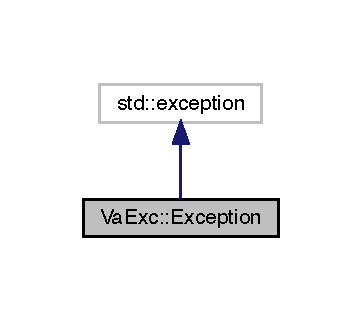
\includegraphics[width=174pt]{class_va_exc_1_1_exception__inherit__graph}
\end{center}
\end{figure}


Collaboration diagram for Va\+Exc\+:\+:Exception\+:\nopagebreak
\begin{figure}[H]
\begin{center}
\leavevmode
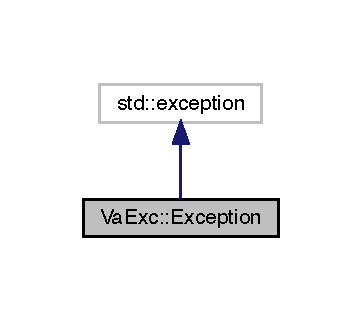
\includegraphics[width=174pt]{class_va_exc_1_1_exception__coll__graph}
\end{center}
\end{figure}
\subsection*{Public Member Functions}
\begin{DoxyCompactItemize}
\item 
\mbox{\Hypertarget{class_va_exc_1_1_exception_af13faa3d0a78c38c70252255aaf926ec}\label{class_va_exc_1_1_exception_af13faa3d0a78c38c70252255aaf926ec}} 
{\footnotesize template$<$class... Args$>$ }\\{\bfseries Exception} (Args \&\&... args) noexcept
\item 
\mbox{\Hypertarget{class_va_exc_1_1_exception_a43f332b702c6e9812f37193b8512bb62}\label{class_va_exc_1_1_exception_a43f332b702c6e9812f37193b8512bb62}} 
virtual const char $\ast$ {\bfseries what} () const noexcept override
\end{DoxyCompactItemize}


\subsection{Detailed Description}
The \hyperlink{class_va_exc_1_1_exception}{Exception}. 

\hyperlink{class_va_exc_1_1_exception}{Exception} is just like std\+::exception, but it gives more information on the error (func, line, file), Exception\+::what() can print arguments in any order (\mbox{[}msg, line, func\mbox{]} or \mbox{[}func, msg, line\mbox{]}), \hyperlink{class_va_exc_1_1_exception}{Exception} is inherited from std\+::exception (thus, it is a std\+::exception), \hyperlink{class_va_exc_1_1_exception}{Exception} supports formatted strings, just like std\+::printf.

\begin{DoxySeeAlso}{See also}
operator\char`\"{}\char`\"{}\+\_\+msg(), operator\char`\"{}\char`\"{}\+\_\+file(), operator\char`\"{}\char`\"{}\+\_\+func(), operator\char`\"{}\char`\"{}\+\_\+line(), \hyperlink{struct_va_exc_1_1__wrappers_1_1_arg_msg_ad7bb2c449c64e2ea7fb38cff28075705}{\+\_\+wrappers\+::\+Arg\+Msg\+::\+Arg\+Msg()}, V\+A\+E\+X\+C\+\_\+\+P\+OS
\end{DoxySeeAlso}
\begin{DoxyParagraph}{Examples}

\begin{DoxyCode}
\textcolor{keywordflow}{try}
\{
    \textcolor{keyword}{using namespace }\hyperlink{namespace_va_exc}{VaExc};

    \textcolor{comment}{// ArgMsg is implemented via std::sprintf, so formatting is the same.}
    \textcolor{keywordflow}{throw} \hyperlink{class_va_exc_1_1_exception}{Exception}(\hyperlink{struct_va_exc_1_1__wrappers_1_1_arg_msg}{ArgMsg}(\textcolor{stringliteral}{"Error code: %d"}, error\_code), VAEXC\_POS);

    ...
\}
\textcolor{keywordflow}{catch} (\hyperlink{class_va_exc_1_1_exception}{Exception}& exc)
\{
    \textcolor{keywordflow}{throw} \hyperlink{class_va_exc_1_1_exception}{Exception}(\textcolor{stringliteral}{"Exception occured!!!"}, exc);
\}

...

try
\{
    \textcolor{keyword}{using namespace }\hyperlink{namespace_va_exc}{VaExc};

    \textcolor{keywordflow}{throw} \hyperlink{class_va_exc_1_1_exception}{Exception}(\textcolor{stringliteral}{"Aaaa!"}\_msg, \textcolor{stringliteral}{"Fuuuunc!11!1"}\_func, 1111\_line);

    ...
\}
\textcolor{keywordflow}{catch} (std::exception& exc) \textcolor{comment}{// Also catches Exception}
\{
    \textcolor{keywordflow}{throw} \hyperlink{class_va_exc_1_1_exception}{Exception}(\textcolor{stringliteral}{"Exception occured!!!"}, VAEXC\_POS, exc);
\}
\end{DoxyCode}
 
\end{DoxyParagraph}


The documentation for this class was generated from the following file\+:\begin{DoxyCompactItemize}
\item 
/\+Users/vladislav\+\_\+aleinik/\+Dropbox/\+Programming/cpp/2016-\/2017/my\+\_\+exception\+\_\+improved/src/Va\+Exception.\+hpp\end{DoxyCompactItemize}

%--- End generated contents ---

% Index
\backmatter
\newpage
\phantomsection
\clearemptydoublepage
\addcontentsline{toc}{chapter}{Index}
\printindex

\end{document}
